\chapter{Упражнения по работе с пользовательскими функциями \unf}

Освоить работу с расчетными функциями \unf{} можно выполняя упражнения описанные в данном разделе и изучая устройство тестовых расчетных модулей. Упражнения демонстрируют некоторые типовые приемы работы с пользовательскими функциями \unf{}. На основе этих приемов можно создать свои расчетные модули решающие специфические задачи пользователя. Примеры не являются исчерпывающими. Варианты работы с расчетными модулями \unf{} не ограничиваются описанными приемами. Цель данного описания - помочь сделать первые шаги в проведении расчетов.
Упражнения помогут: 
\begin{itemize}	
	\item 	освоить принципы работы c пользовательскими функциями \unf{} 
	\item 	изучить основы проведения инженерных расчетов в области добычи нефти
\end{itemize}

\section{Трюки и лайфхаки при работе в excel с функциями \unf{}}
Знание некоторых трюков может сильно упростить работу с пользовательскими функциями \unf{}.
\begin{enumerate}
	\item Для работы с примером должна быть запущена надстройка \unf{}. Убедиться, что надстройка запущена можно найдя вкладку Unifloc в панели меню Excel, рис. \ref{ris:excel_unifloc_tab}.
	
	\begin{figure}[h!]
		\center{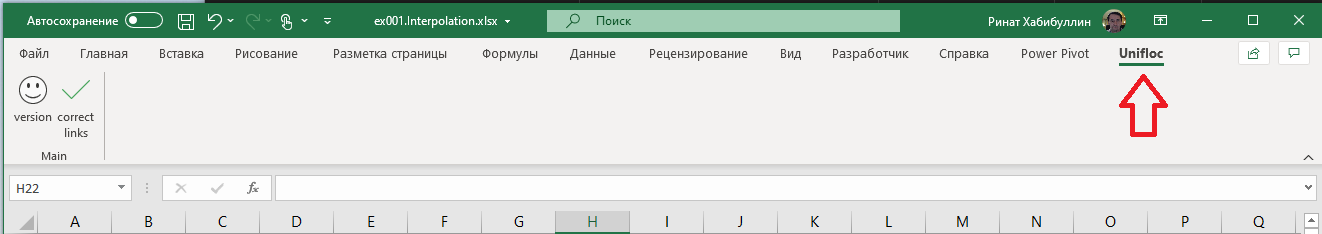
\includegraphics[width=0.8\linewidth]{excel_unifloc_tab}}
		\caption{Открытая панель Unifloc}
		\label{ris:excel_unifloc_tab}
	\end{figure}
	
	\item При необходимости вывести массив значений как результат расчета функций \mintinline{vb.net}{crv_solve} или \mintinline{vb.net}{crv_intersection} используйте комбинацию клавиш \texttt{Cntrl+Shift+Enter} или динамические массивы\footnote{подробнее про динамические массивы (dynamic arrays) можно посмотреть в интернете, например - https://www.planetaexcel.ru/techniques/2/9112/}(для новых версий Excel). Если для динамических массивов требуется подавить вывод массива - используйте знак @ в строке вызова, например как \mintinline{vb.net}{=@crv_solve(...)}.
	
	\item Все названия функций \unf{} начинаются с префикса. Это позволяет быстро искать необходимые функции. При запущенной надстройке достаточно начать вводить в ячейку формулу, например ввести \texttt{=PVT} как Excel откроет выпадающий список с подсказкой, показывающий возможные варианты названий функций (смотри рис. \ref{ris:Ex10_2}). 
	
	\begin{figure}[h!]
		\center{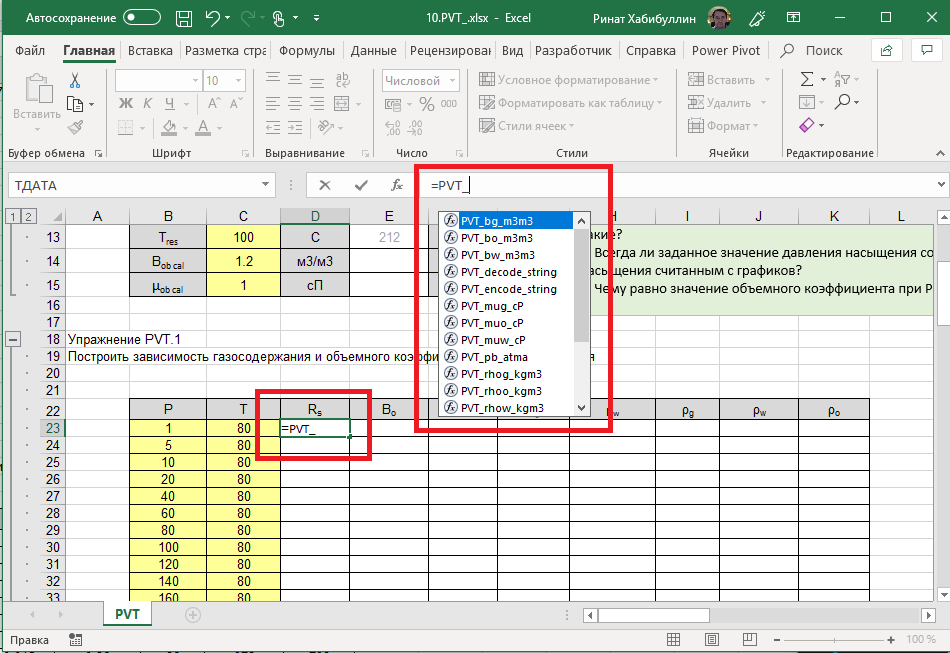
\includegraphics[width=0.8\linewidth]{Ex10_2}}
		\caption{Выпадающий список с подсказками названий функции}
		\label{ris:Ex10_2}
	\end{figure}
	
	\item 	Из выпадающего списка выберите функцию \texttt{=PVT\_Rs\_m3m3(} после чего нажмите кнопку $f_x$ "вставить функцию"  слева от строки формул. Это вызовет окно задания параметров функции, в котором будут указаны все параметры, которые необходимо ввести (смотри рис. \ref{ris:Ex10_3}). В этом окно можно задать необходимые значения параметров или указать ссылки на соответствующие ячейки. Для "хороших" функций в окне задания параметров функции будут подсказки. Также в окне задания параметров можно сразу видеть результат расчета если задан достаточный набор параметров.
	
	\begin{figure}[h!]
		\center{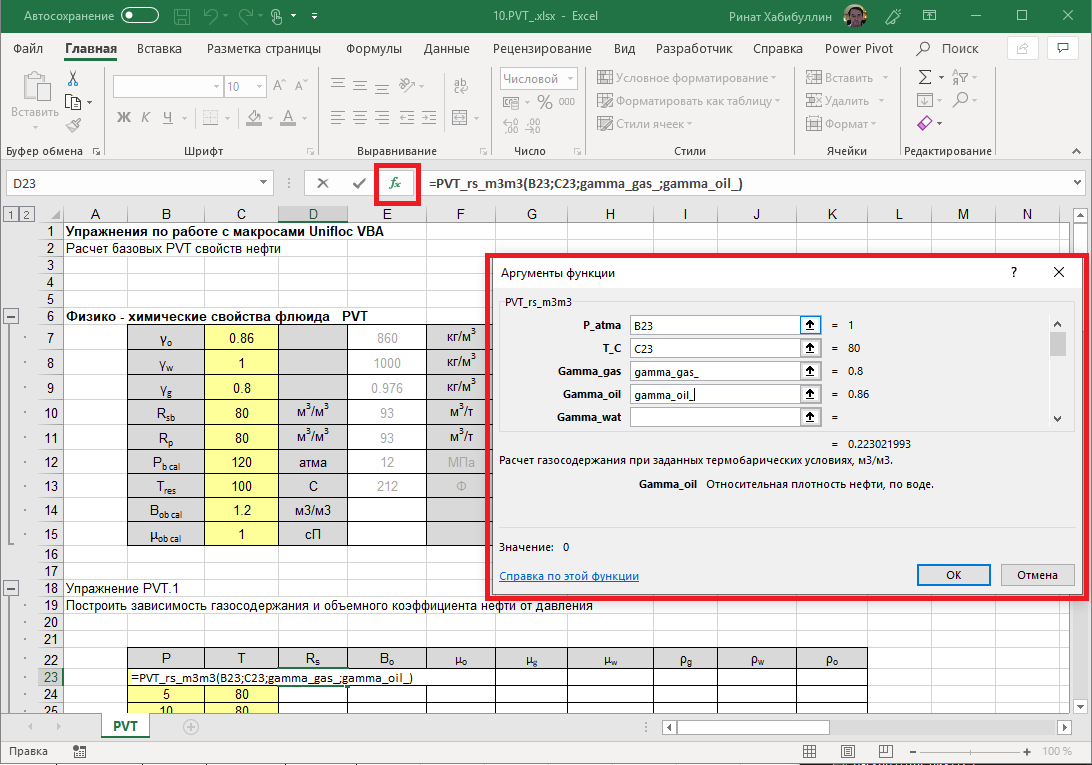
\includegraphics[width=0.8\linewidth]{Ex10_3}}
		\caption{Окно ввода аргументов функции}
		\label{ris:Ex10_3}
	\end{figure}
	
	\item После ввода всех параметров и нажатия кнопки ОК в ячейке должен отобразиться результат расчета. Воспользовавшись инструментом "Влияющие ячейки" на вкладке "Формулы"\ можно отследить на какие ячейки ссылается введенная формула (смотри рис. \ref{ris:Ex10_4})
	\begin{figure}[h!]
		\center{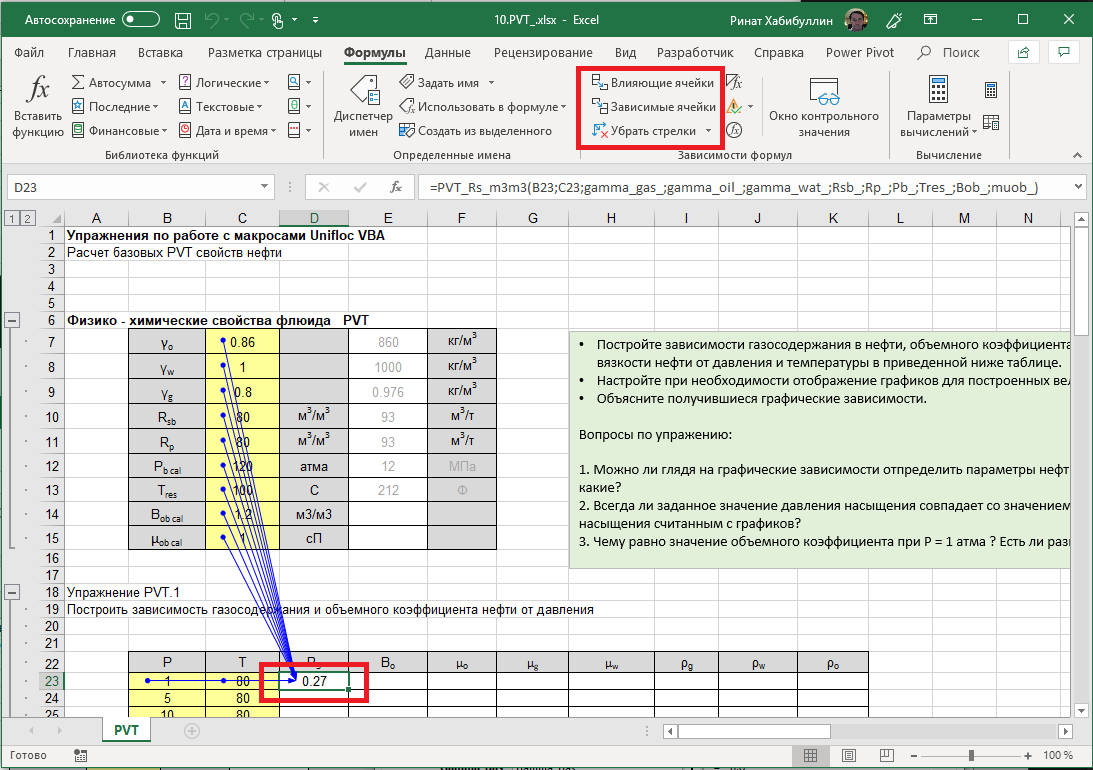
\includegraphics[width=0.8\linewidth]{Ex10_4}}
		\caption{Результат вызова пользовательской функции с отображение влияющих ячеек}
		\label{ris:Ex10_4}
	\end{figure}
\end{enumerate}


\section{Работа с таблично заданными кривыми}
Инженерный анализ требует умения ловко работать с графическими данными - кривыми, картами, кросс плотами и графиками. Кроме отображения графических данных, что легко делается стандартными программами - часто требует проводить по ним расчеты. Набор функций \unf{} для работы с таблично заданными кривыми может оказать полезными для этих целей. 

Функции \unf{} для работы с таблично заданными кривыми начинаются с префикса \mintinline{vb.net}{crv_}, от слова curve. Доступна функциональность
\begin{itemize}	
	\item интерполяции различными методами (работает и экстраполяция)
	\item поиска решения уравнения вида $f(x) = с$ где функция $f(x)$ задана таблицей (ищется решение для линейной аппроксимации)
	\item поиска пересечений двух кривых заданных таблицами (ищется решение для линейно аппроксимации)	
\end{itemize}
В коде можно обнаружить еще ряд функций, но они не будут описываться в данном руководстве, хотя по ним можно найти примеры в папке \texttt{examples} репозитория.

\subsection{Интерполяция линейная и сплайнами}
Файл примера \texttt{ex001.Interpolation.xlsx} можно найти в папке \texttt{exercises} репозитория \unf{}.

\begin{enumerate}
	\item Для работы с примером должна быть запущена надстройка \unf{}. Убедиться, что надстройка запущена можно найдя вкладку Unifloc в панели меню Excel, рис. \ref{ris:excel_unifloc_tab}.
	

	
	\item Откройте файл с упражнением \texttt{ex001.Interpolation.xlsx} (смотри рис. \ref{ris:Ex001_1}).
	
	\begin{figure}[h!]
		\center{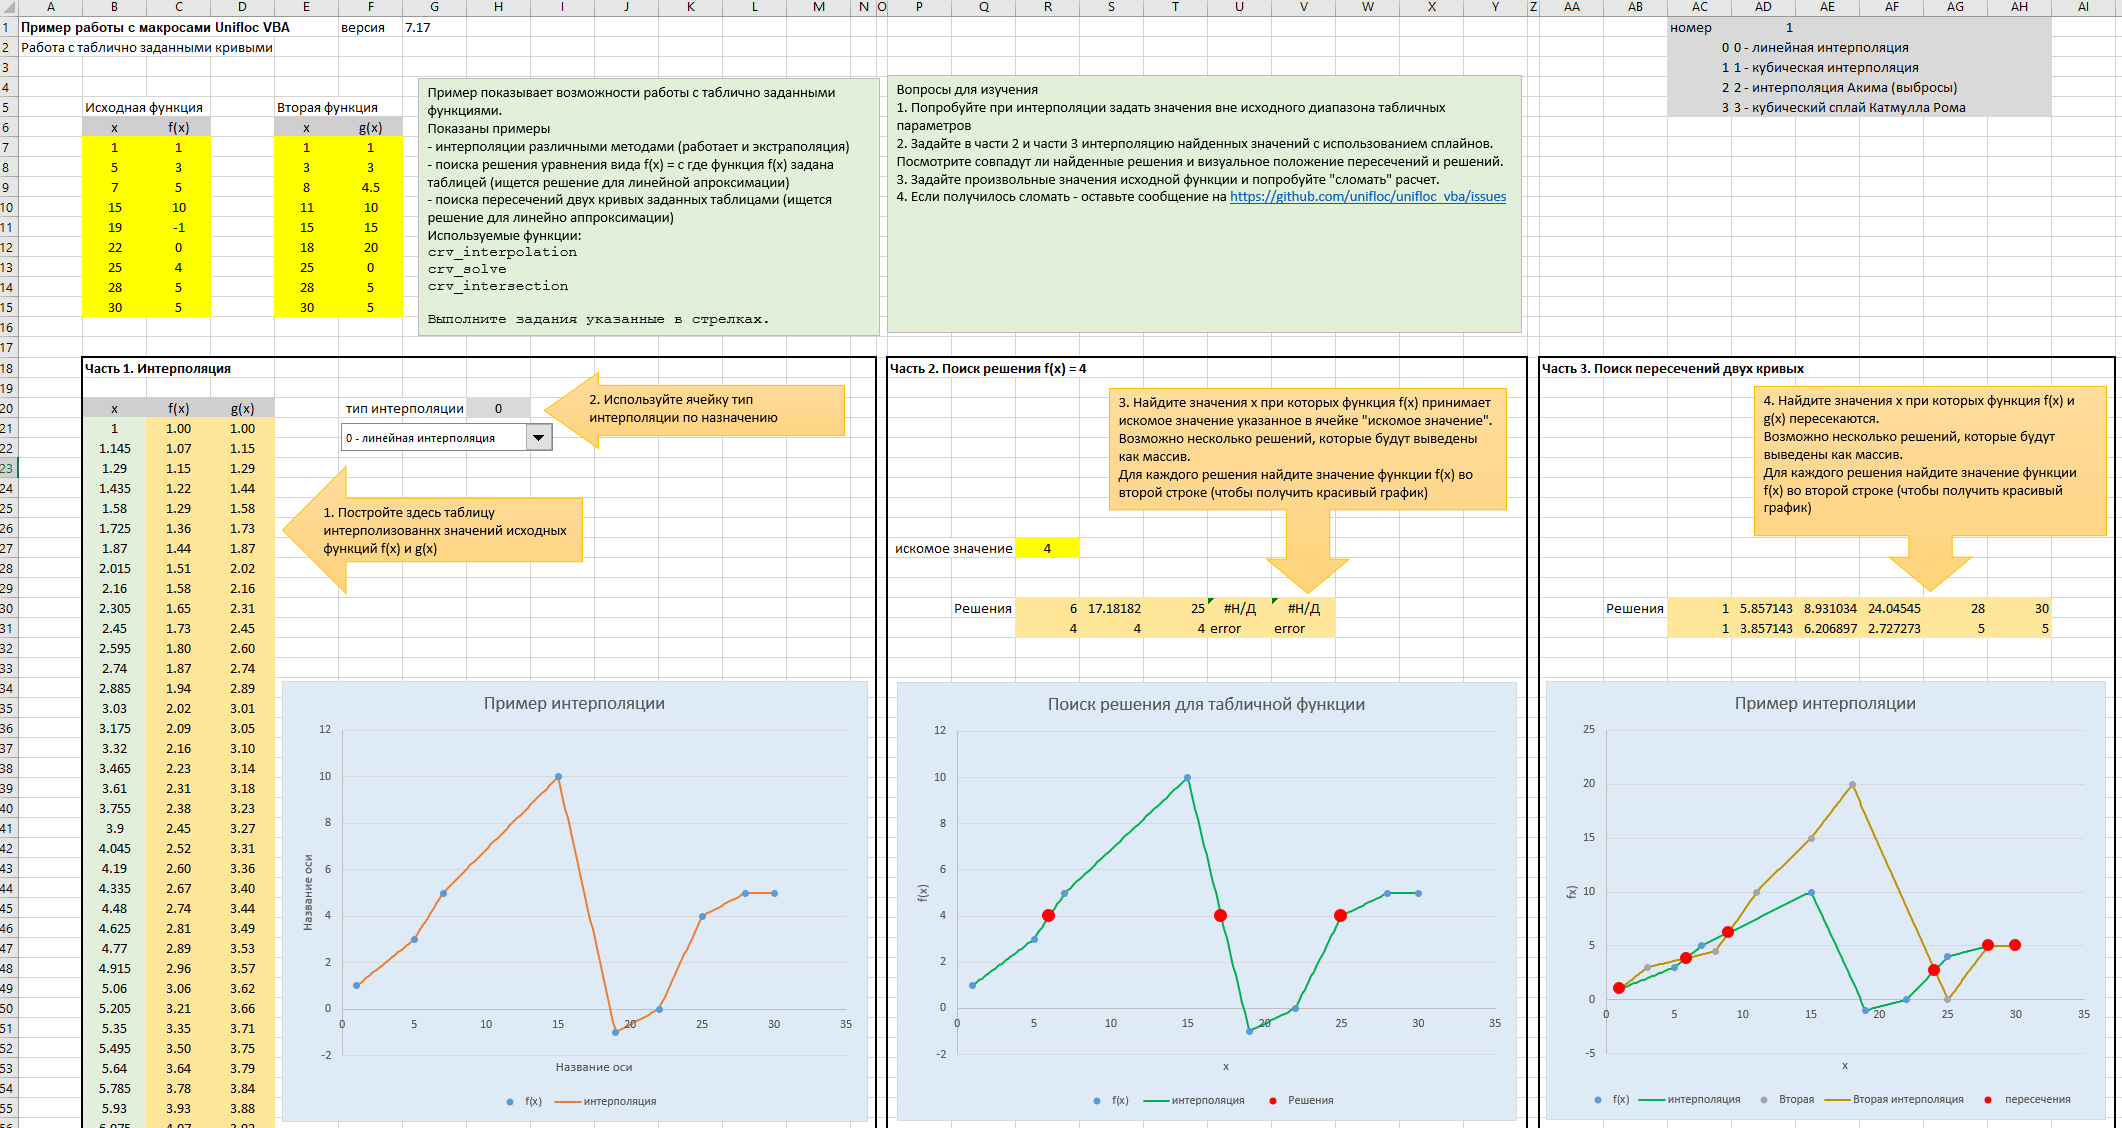
\includegraphics[width=1\linewidth]{Ex001_1}}
		\caption{Упражнение \texttt{ex001.Interpolation.xlsx} со всеми заполненными полями}
		\label{ris:Ex001_1}
	\end{figure}
	
	Пример разделен на три части: Часть 1. Интерполяция; Часть 2. Поиска решения $f(x)=c$; Часть 3.Поиск пересечения двух кривых.
	
	\item Выполните задания указанные в стрелках (последовательность выполнения по номерам стрелок). При этом должны автоматически построиться графики как на рисунке \ref{ris:Ex001_1}).
	

	
	\item Постарайтесь ответить на вопросы в блоке "Вопросы для изучения"

\end{enumerate}

\section{Расчет базовых PVT свойств флюидов}

Расчет физико химических свойств пластовых флюидов (PVT параметров) лежит в основе всех расчетов систем нефтедобычи. При решении прикладных задач редко возникает необходимость расчета PVT свойств непосредственно, однако понимание принципа их расчета, а особенно зависимости результатов расчета от исходных данных важно.
   
Для выполнения упражнения используйте файл "ex010.PVT.xlsx"

\begin{enumerate}

	\item Откройте файл с упражнением \texttt{10.PVT.xlsx} (смотри рис. \ref{ris:Ex10_1}).
	
	\begin{figure}[h!]
		\center{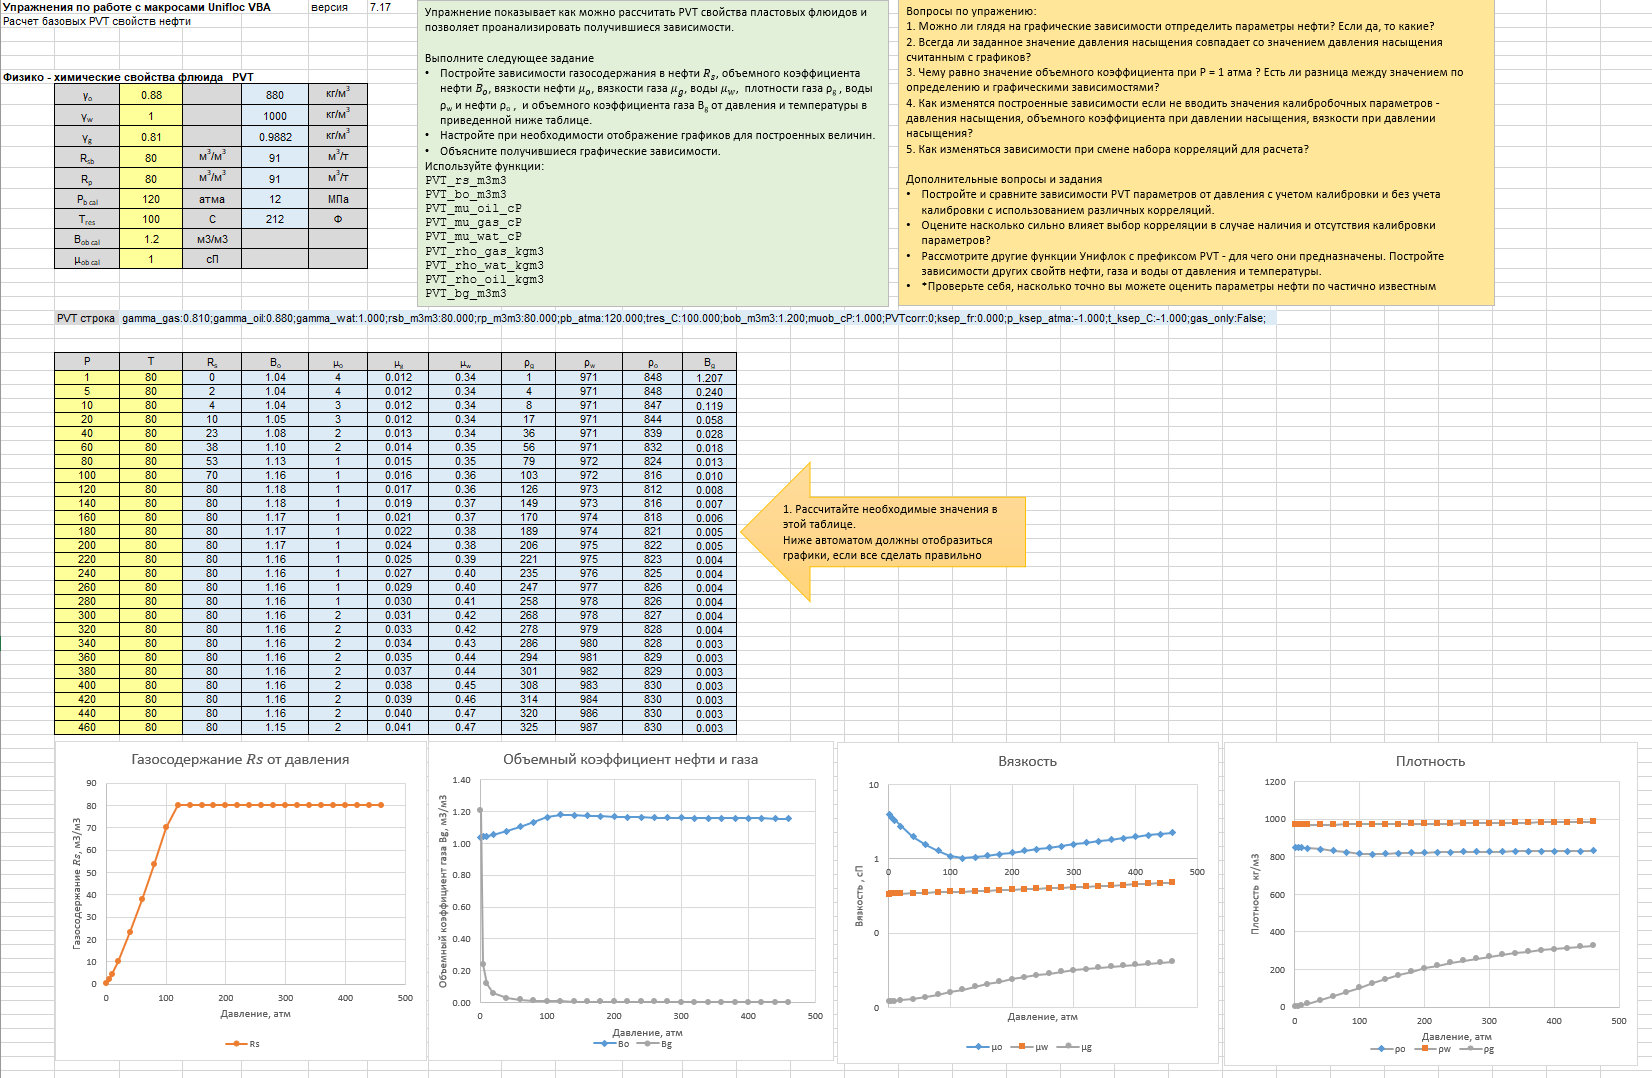
\includegraphics[width=1\linewidth]{Ex10_1}}
		\caption{Упражнение \texttt{ex010.PVT.xlsx} со всеми заполненными полями.}
		\label{ris:Ex10_1}
	\end{figure}
	
	\item Выполните задания указанные в описании. Задания просты -- требуется рассчитать таблицу значений для построения графиков и провести анализ построенных графиков. Названия необходимых функций указаны в описании  \ref{ris:Ex10_1}). Вопросы по упражнению помогут вам провести анализ. Текст заданий не приводится в описании, так как файлы упражнений первичны. Любые изменения скорее будут вноситься в файлы с заданиями, нежели в описание.
	
	\item Ответьте на вопросы по упражнению приведенные в рабочей книге.
	 
\end{enumerate}

\section{Расчет свойств потока флюидов}

PVT функции описывают свойства флюидов. Можно представить себе, что они описывают свойства флюидов находящихся в PVT бомбе - устройстве для отбора проб. В этом случае флюиды неподвижны и находятся в равновесном состоянии. На практике приходится иметь дело с флюидами двигающимися в скважине или трубопроводе - с потоком флюидов. В потоке флюидов добавляются дополнительные параметры -- расход флюидов или дебит $Q_{liq}, Q_g$ и обводненность $f_w$ -- показатель показывающий объемную долю воды в потоке. 
Функции работающие с потоками в \unf{} имеют префикс \mintinline{vb.net}{MF_}. Префикс должен намекать на многофазность потока и на самом деле плох с лингвистической точки зрения (multiphase - has no F letter), но удобен с программистской точки зрения и уже поздно его менять.

Файл примера \mintinline{vb.net}{ex011.Gas_fraction.xlsx} можно найти в папке \texttt{exercises} репозитория \unf{}.

\begin{enumerate}
	
	\item Откройте файл с упражнением \texttt{10.PVT.xlsx} (смотри рис. \ref{ris:Ex11_1}).
	
	\begin{figure}[h!]
		\center{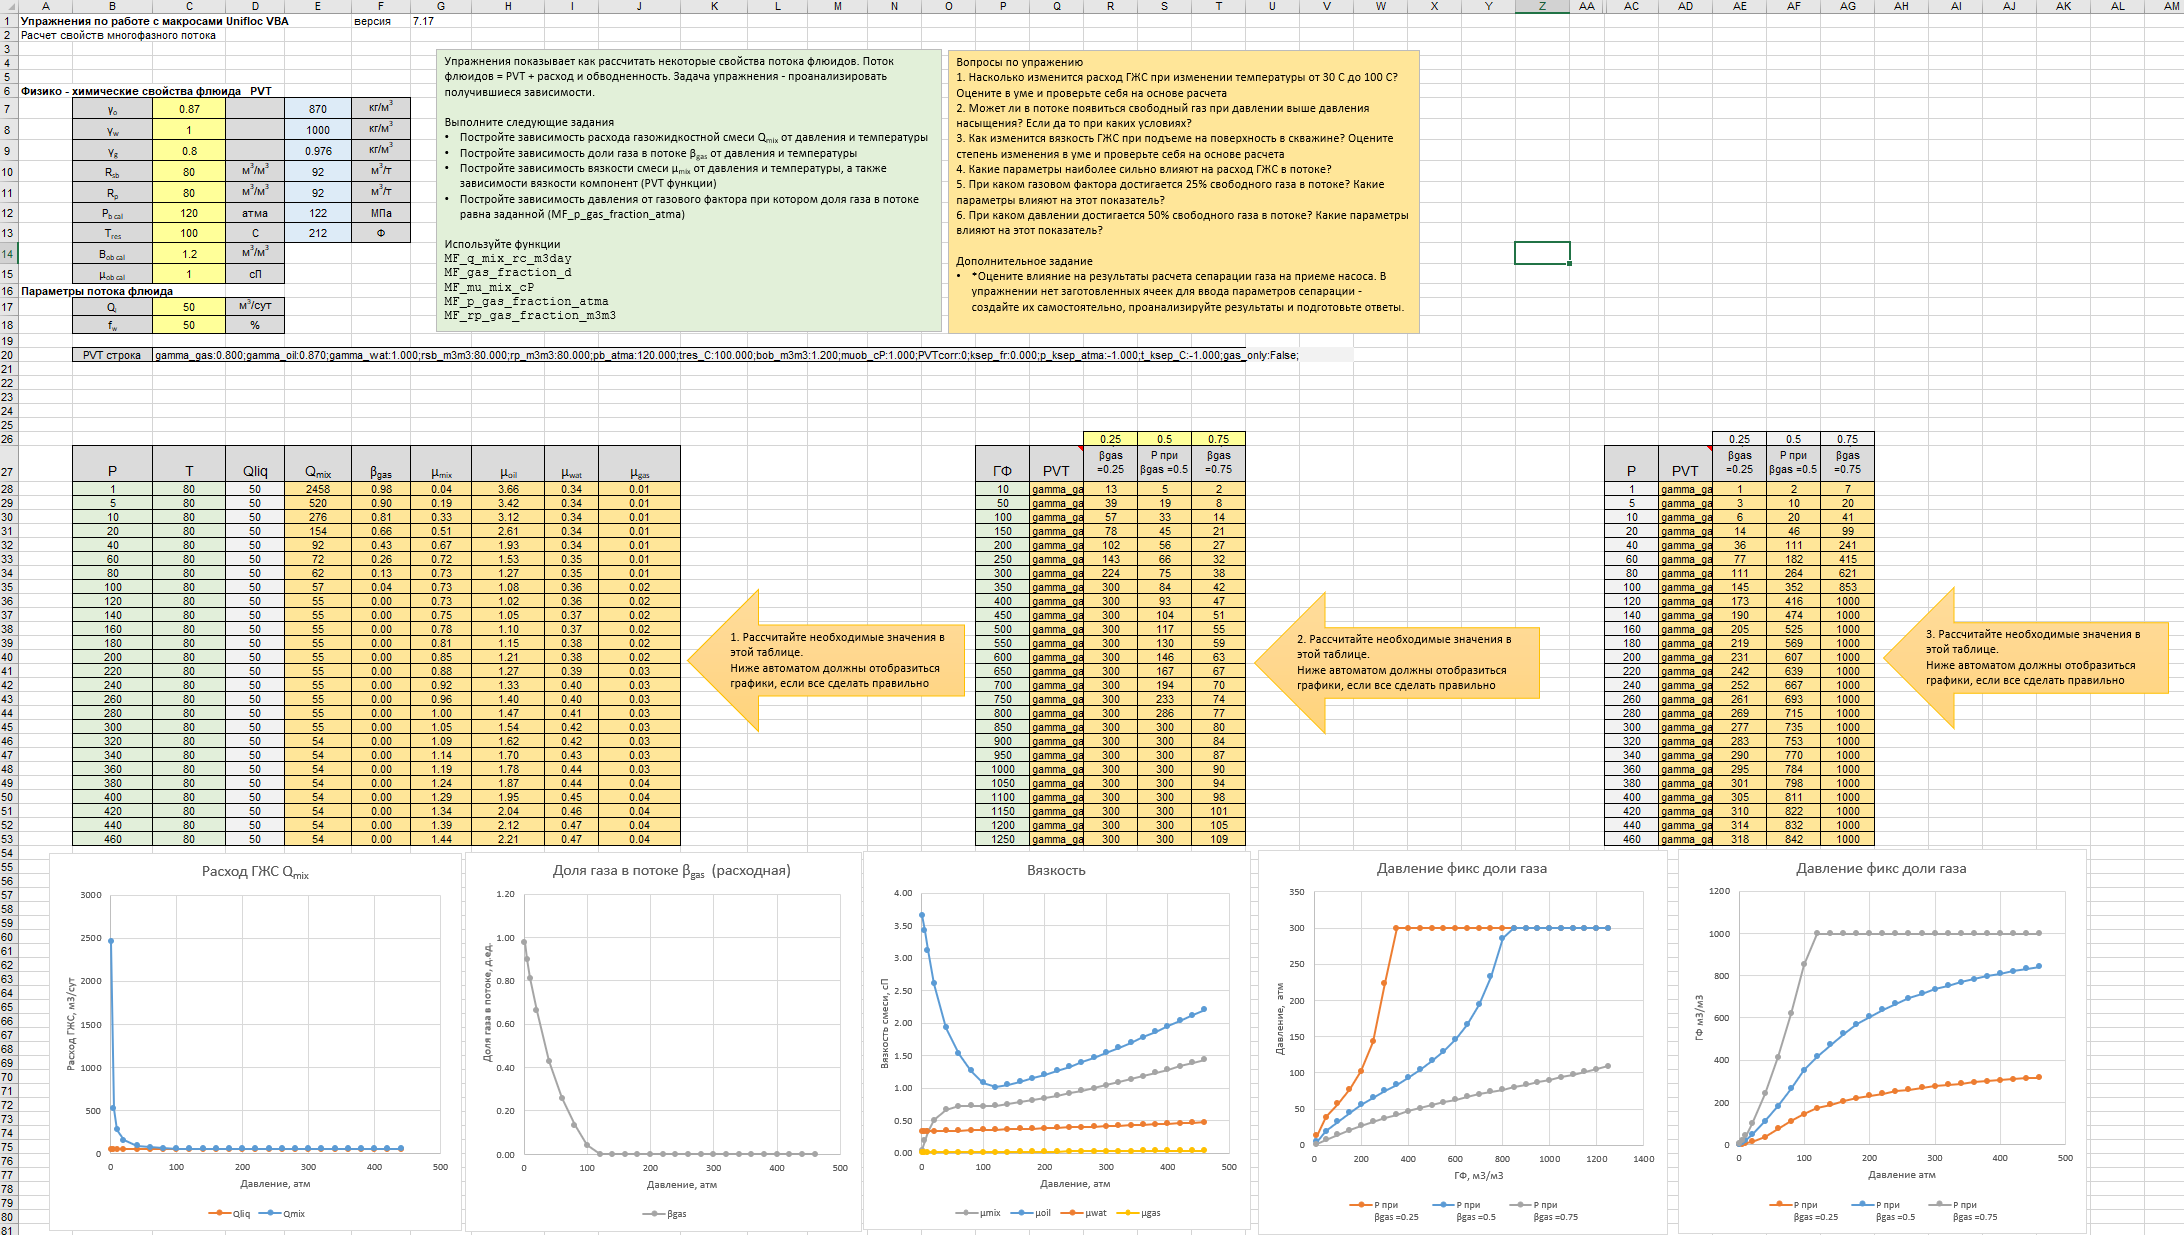
\includegraphics[width=1\linewidth]{Ex11_1}}
		\caption{Упражнение \mintinline{vb.net}{ex011.Gas_fraction.xlsx} со всеми заполненными полями }
		\label{ris:Ex11_1}
	\end{figure}
	
	\item Выполните задания указанные в описании. Задания просты -- требуется рассчитать три таблицы значений для построения графиков и провести анализ построенных графиков. Названия необходимых функций указаны в описании  \ref{ris:Ex11_1}). Вопросы по упражнению помогут вам провести анализ. Текст заданий не приводится в описании, так как файлы упражнений первичны. Любые изменения скорее будут вноситься в файлы с заданиями, нежели в описание.
	
	\item Ответьте на вопросы по упражнению приведенные в рабочей книге.
	
	\item Выполните дополнительное задание, если чувствуете силы. В дополнительном задании говорится о сепарации газа на приеме насоса. Имеется в виду следующее - если у нас есть пластовые флюиды, свойства которых мы знаем и можем задать, то после сепарации части свободного газа, что часто происходит на скважинном насосе, свойства флюида изменятся. Изменится его эффективное давление насыщения (потому что мы убрали часть газа) и газосодержание при давлении насыщения. И соответственно поплывут и остальные свойства. Это можно учесть задав в \mintinline{vb.net}{PVT_Encode()} три параметра - коэффициент сепарации газа $K_{sep}$, давление при которой произошла сепарации $P_{sep}$ и температуру при которой произошла сепарация $T_{sep}$. Подробнее про это можно найти в соответствующих разделах (поэтому тут это задание дополнительное).
	
\end{enumerate}

\section{Расчет производительности скважины}

Стационарная модель притока к скважине (закон Дарси с поправкой Вогеля) - одна из самых простых и распространенных моделей, широко применяемая в индустрии. \unf{} содержит функции позволяющие упростить расчет индикаторной кривой. Такие функции имеют префикс \mintinline{vb.net}{IPR_} от Inflow Performance Relationship.

Файл примера \mintinline{vb.net}{ex020.IPR.xlsx} можно найти в папке \texttt{exercises} репозитория \unf{}.

\begin{enumerate}
	
	\item Откройте файл с упражнением \texttt{ex020.IPR.xlsx} (смотри рис. \ref{ris:Ex20_1}).
	
		\begin{figure}[h!]
			\center{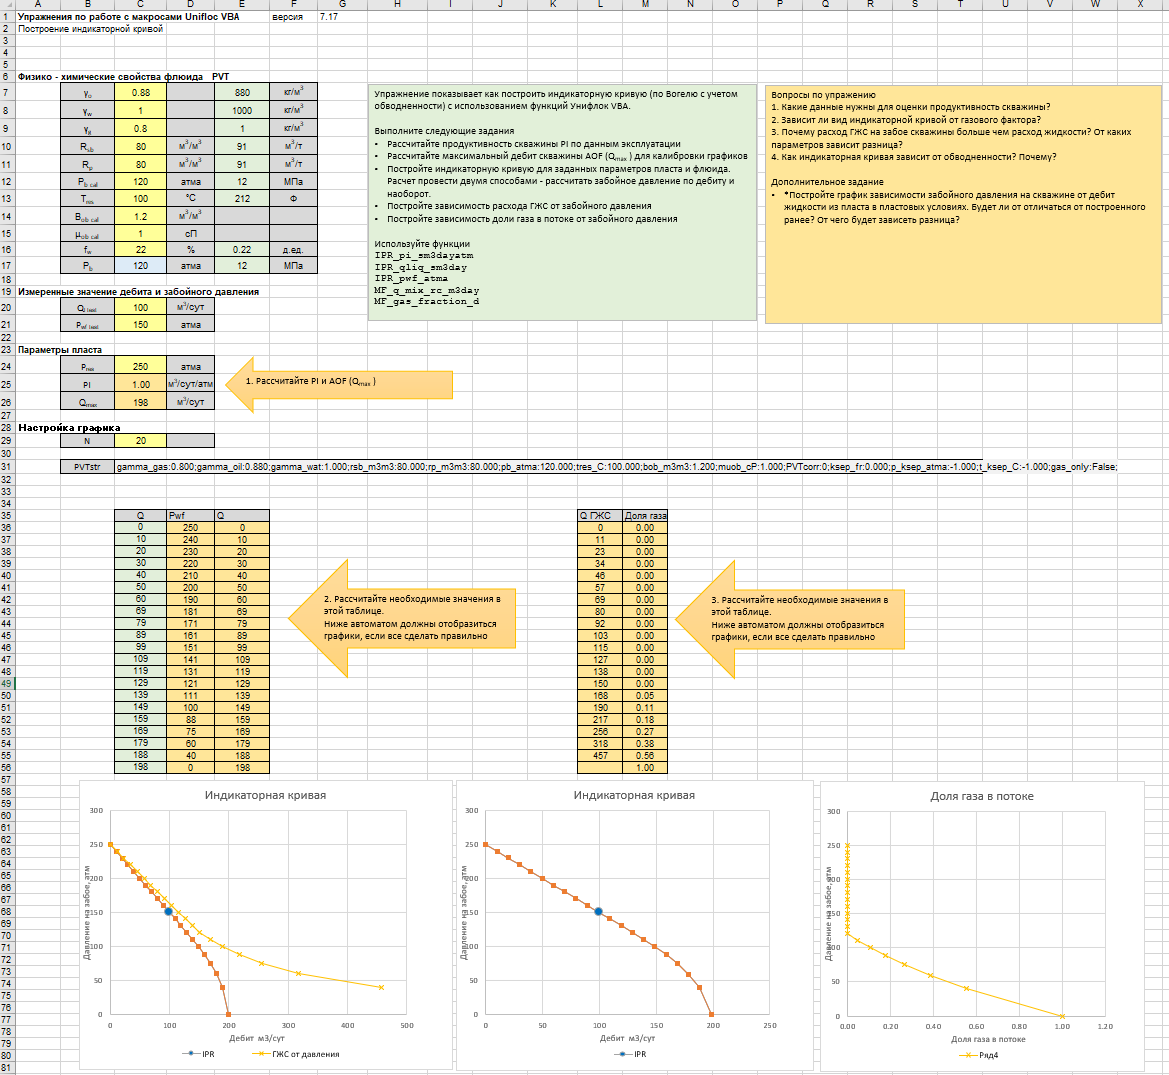
\includegraphics[width=1\linewidth]{Ex20_1}}
			\caption{Упражнение \mintinline{vb.net}{ex020.IPR.xlsx} со всеми заполненными полями }
			\label{ris:Ex20_1}
		\end{figure}

	\item Выполните задания указанные в описании. Задания просты -- требуется рассчитать три таблицы значений для построения графиков и провести анализ построенных графиков. Названия необходимых функций указаны в описании  \ref{ris:Ex11_1}). Вопросы по упражнению помогут вам провести анализ. Текст заданий не приводится в описании, так как файлы упражнений первичны. Любые изменения скорее будут вноситься в файлы с заданиями, нежели в описание.
	
	\item Ответьте на вопросы по упражнению приведенные в рабочей книге.
	
	\item Выполните дополнительное задание, если чувствуете силы.

\end{enumerate}

Коэффициент продуктивности $PI$ скважины рассчитывается в ячейке С25 по замеренным данным  с помощью функции

{ \small  \texttt{=IPR\_PI\_sm3dayatm(qltest\_;Pwftest\_;Pres\_;fw\_;Pb\_)}}

А максимальный дебит $Q_{max}$ при максимальной депрессии с забойным давлением равным нулю

{ \small  \texttt{=IPR\_Qliq\_sm3Day(PI\_;Pres\_;0;fw\_;Pb\_)}}




\section{Расчет штуцера}

Для контроля дебита и/или давления на добывающих скважинах вблизи устья может устанавливаться штуцер. Для штуцера, как для любого гидравлического элемента, возможно 4 варианта расчета - расчет давления по потоку, расчет давления против потока, расчет потока по давлениям и настройка модели штуцера по известным давлениям и потоку. В упражнении демонстрируются все варианты расчета. 

Файл примера \mintinline{vb.net}{ex040.MF_choke.xlsx} можно найти в папке \texttt{exercises} репозитория \unf{}.

\begin{enumerate}
	
	\item Откройте файл с упражнением \mintinline{vb.net}{ex040.MF_choke.xlsx} (смотри рис.\ref{ris:Ex40_1}).
	
	\begin{figure}[h!]
		\center{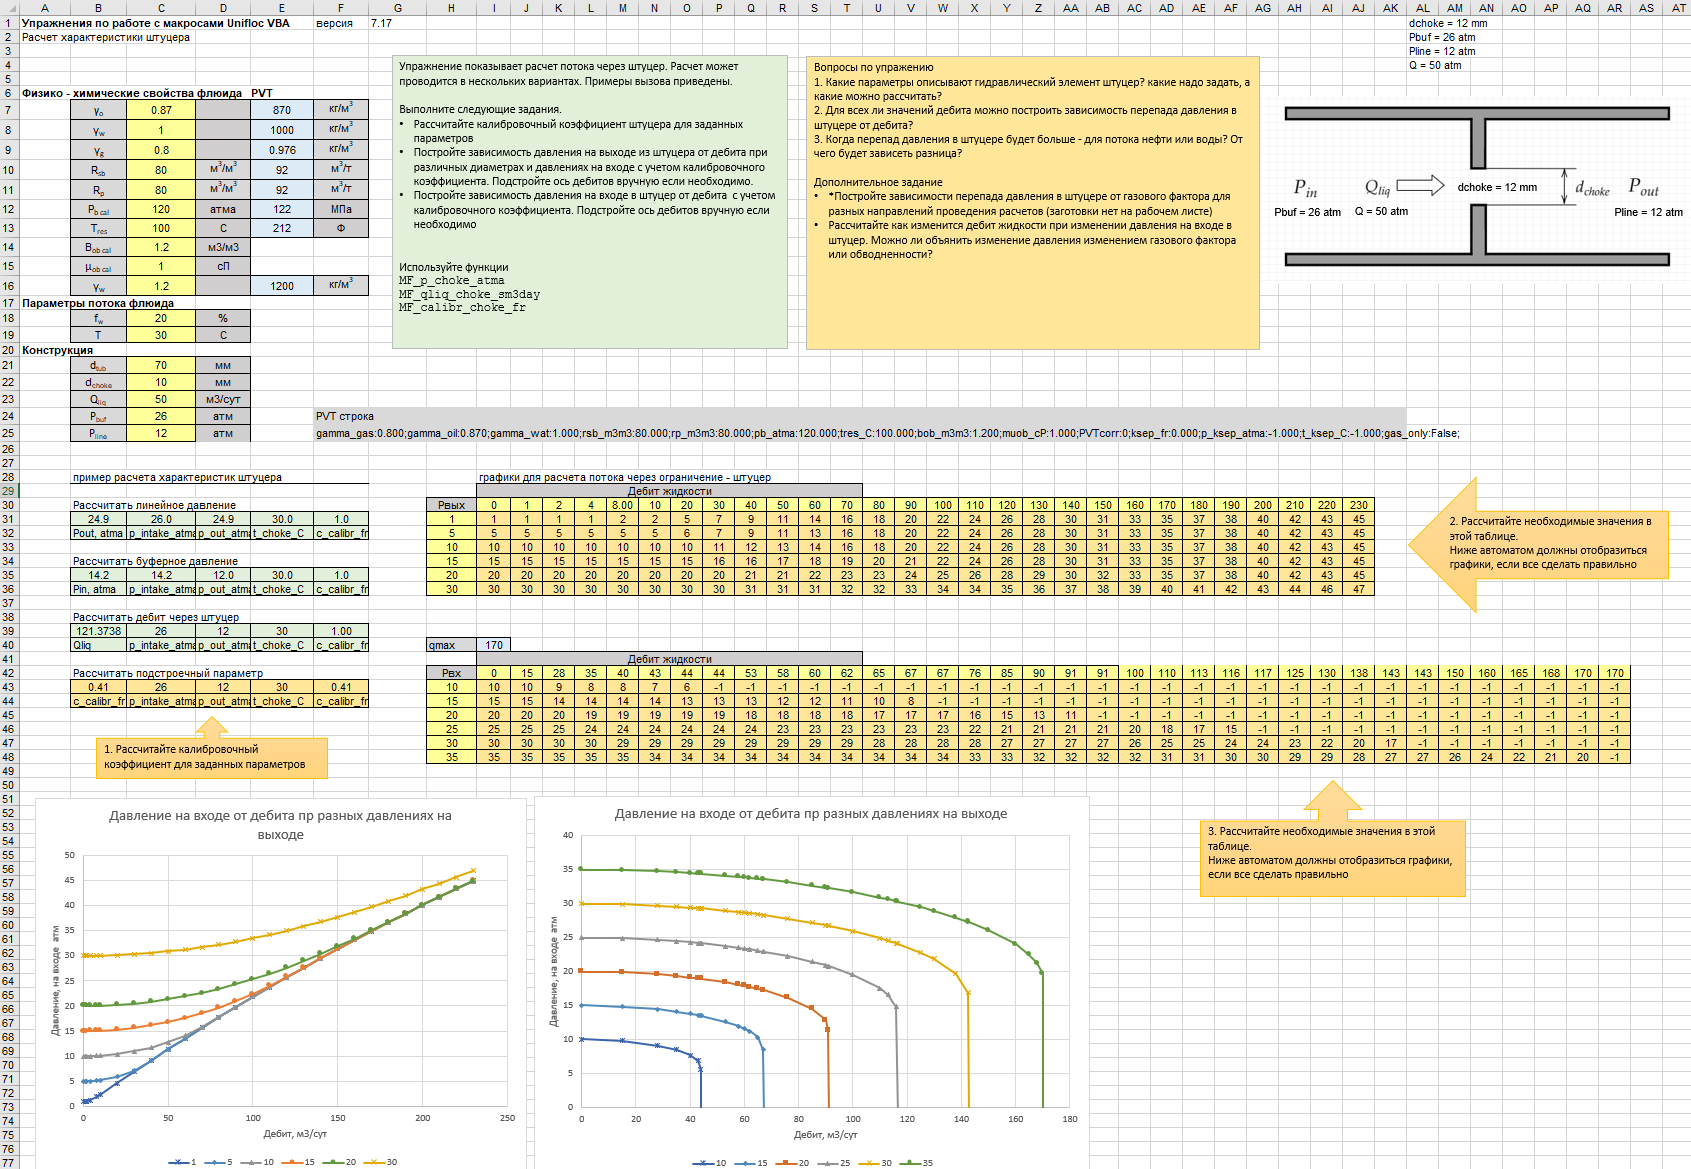
\includegraphics[width=1\linewidth]{Ex40_1}}
		\caption{Упражнение \mintinline{vb.net}{ex040.MF_choke.xlsx} со всеми заполненными полями }
		\label{ris:Ex40_1}
	\end{figure}
	
	\item Выполните задания указанные в описании. Названия необходимых функций указаны в описании  \ref{ris:Ex11_1}). При построении графиков может потребоваться изменить значения дебитов по которым проводится расчет для корректного отображения графиков. Текст заданий не приводится в описании, так как файлы упражнений первичны. Любые изменения скорее будут вноситься в файлы с заданиями, нежели в описание. 
	
	\item Ответьте на вопросы по упражнению приведенные в рабочей книге.
	
	\item Выполните дополнительное задание, если чувствуете силы.
	
\end{enumerate}


\section{Расчет распределения давления в трубе}
Расчет многофазных потоков в трубе - ключевой для анализа работы скважин и скважинного оборудования. Под расчетов трубы подразумевается в первую очередь расчет распределения давления. Иногда требуется рассчитать и распределение температуры. 
На распределение давления в трубе среди прочих параметров влияют режим потока газожидкостной смеси и явление проскальзывание газа. Недоучет данных параметров может привести к значительным ошибкам. Методы для расчета распределения давления можно разделить на две категории: корреляции, полученные экспериментальным путем и механистические модели, в основе которых заложены физические модели.

В \unf{} есть два набора функций для работы с трубой - простые по работе с прямым участком трубы \mintinline{vb.net}{MF_p_pipe} и более сложные по работе с участком трубопровода с учетом рельефа или инклинометрии \mintinline{vb.net}{MF_p_pipeline}

\subsection{Расчет прямолинейного участка трубы. Простой вариант}
Файл примера \mintinline{vb.net}{ex050.MF_pipe.xlsx} можно найти в папке \texttt{exercises} репозитория \unf{}.

\begin{enumerate}
	
	\item Откройте файл с упражнением \mintinline{vb.net}{ex050.MF_pipe.xlsx} (смотри рис.\ref{ris:Ex50_1}).
	
	\begin{figure}[h!]
		\center{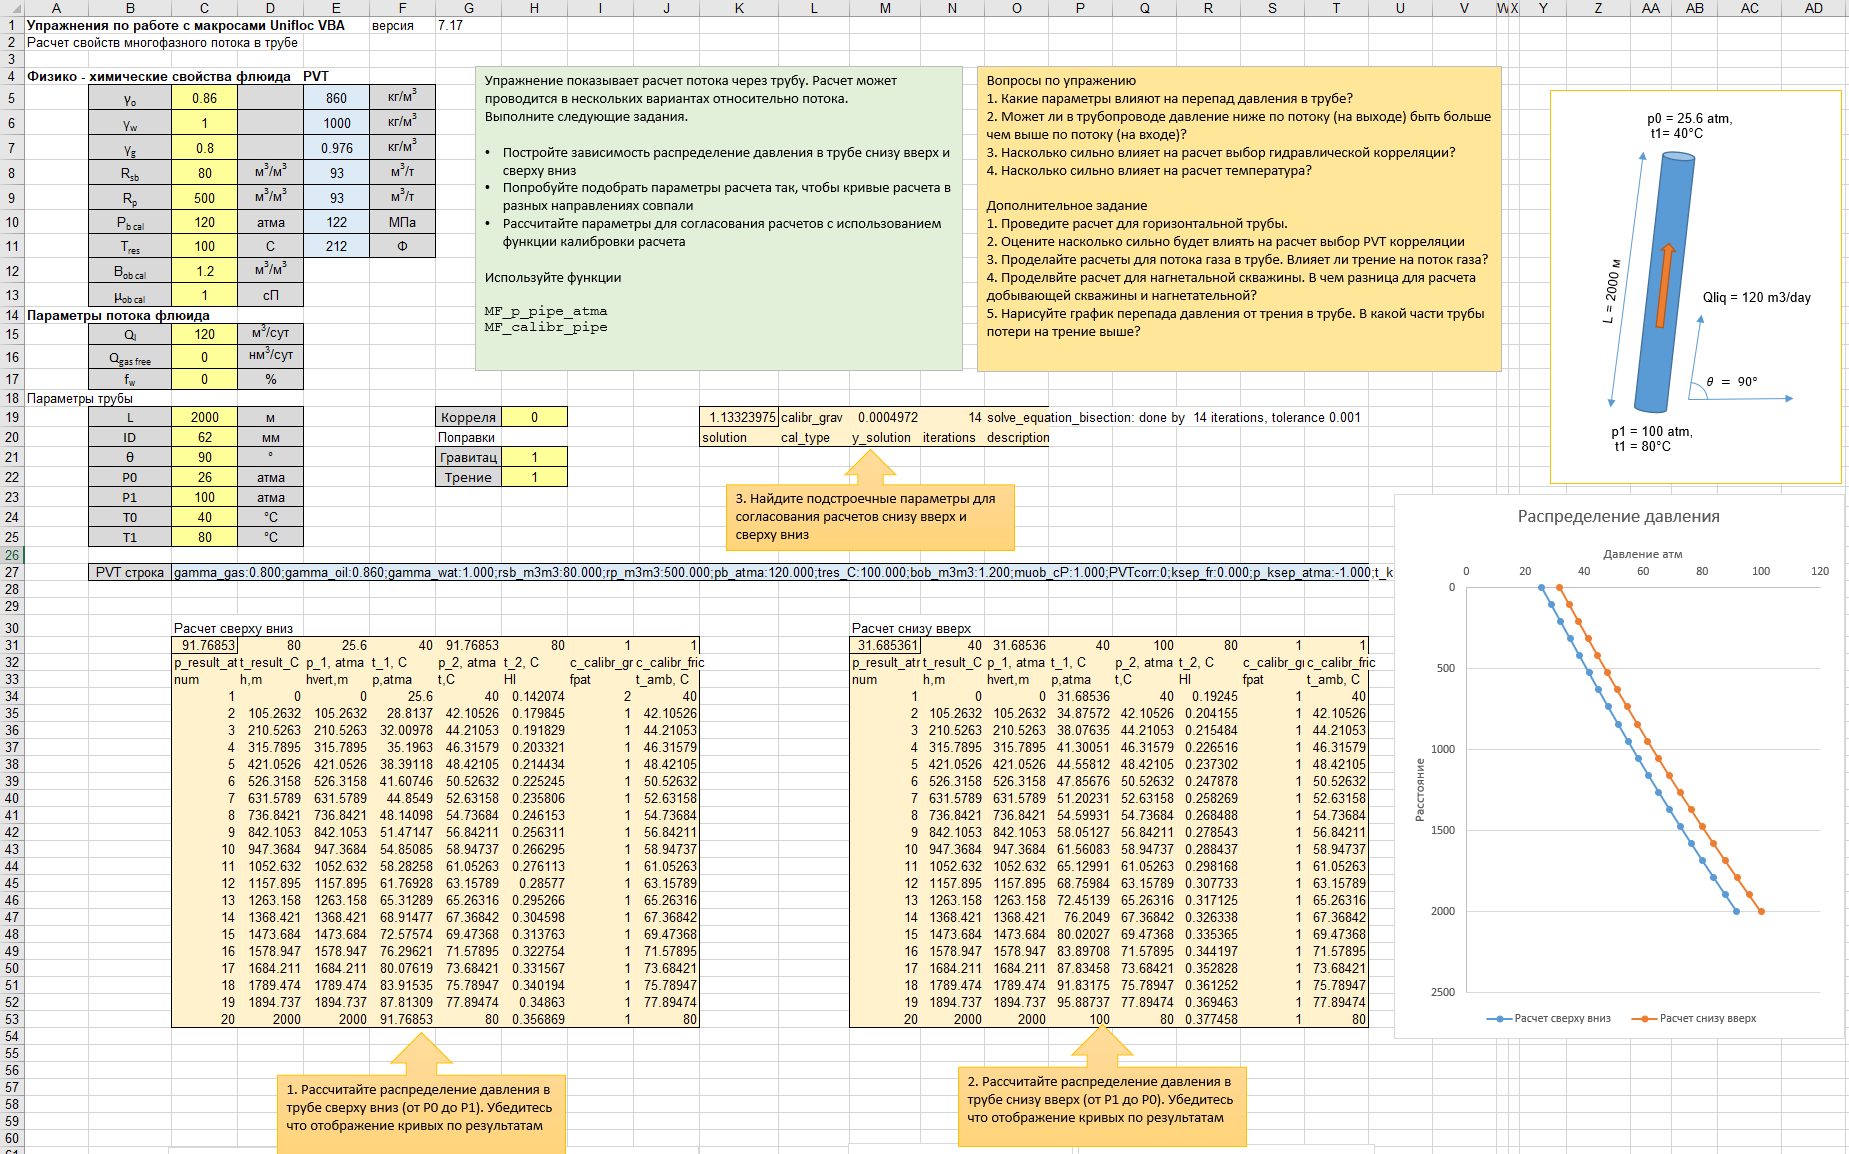
\includegraphics[width=1\linewidth]{Ex50_1}}
		\caption{Упражнение \mintinline{vb.net}{ex050.MF_pipe.xlsx} со всеми заполненными полями }
		\label{ris:Ex50_1}
	\end{figure}
	
	\item Выполните задания указанные в описании. Названия необходимых функций указаны в описании  \ref{ris:Ex50_1}). Текст заданий не приводится в описании, так как файлы упражнений первичны. Любые изменения скорее будут вноситься в файлы с заданиями, нежели в описание. 
	
	\item Ответьте на вопросы по упражнению приведенные в рабочей книге.
	
	\item Выполните дополнительное задание, если чувствуете силы.
	
\end{enumerate}





\section{Расчет коэффициентов сепарации}

Процессы сепарации на приеме погружного оборудования значительно влияют на процесс добычи. Как при естественной, так и при искусственной сепарации (при применении газосепараторов) меняются свойства многофазного потока, уменьшается газлифтный эффект, изменяется режим работы центробежного насоса.

В данном упражнении помимо стандартного определения PVT свойств требуется задать термобарические условия на приеме погружного оборудования (в месте, где происходит сепарация) и конструктивные параметры


\begin{figure}[h!]
	\center{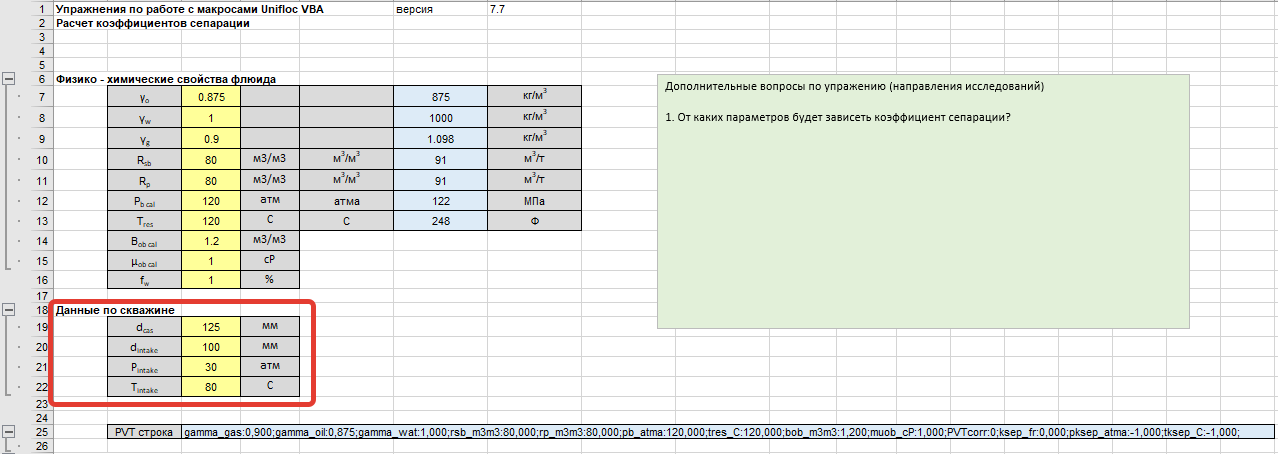
\includegraphics[width=1\linewidth]{Ex60_1}}
	\caption{Исходные данные для сепарации}
	\label{ris:Ex60_1}
\end{figure}

где

$d_{cas}$ - диаметр обсадной колонны, мм

$d_{intake}$ - диаметр приема погружного оборудования, мм

$P_{intake}$ - давление на приеме, атм

$T_{intake}$ - температура на приеме, С

Для вычисления коэффициента естественной сепарации в зависимости от дебита вставьте в ячейку E32 следующую формулу 

{ \small  \texttt{=MF\_ksep\_natural\_d(C32; wc\_; Pintake\_; Tintake\_; Dintake\_; Dcas\_; PVT\_str\_)}}

Для проведения экспериментов по влиянию изменения диаметра обсадной колонны воспользуйтесь в ячейке F32 формулой

{ \small  \texttt{=MF\_ksep\_natural\_d(C32; wc\_; Pintake\_; Tintake\_; Dintake\_; Dcas\_*cf\_dcas\_; PVT\_str\_)}}

При этом в ячейке F30 с помощью коэффициента Вы можете варьировать диаметр обсадной колонны

Для расчета доли газа в газосепараторе применяется функция

{ \small  \texttt{=MF\_gas\_fraction\_d(Pintake\_;Tintake\_;0;PVT\_str\_)*(1-F32)
}}

Коэффициент сепарации газосепаратора

{ \small  \texttt{=MF\_ksep\_gasseparator\_d(gassep\_type;G32;C32)
}}

При этом можно менять тип газосепаратора в ячейке H30

Общий коэффициент сепарации

{ \small  \texttt{=MF\_ksep\_total\_d(E32;H32)
}}

\begin{figure}[h!]
	\center{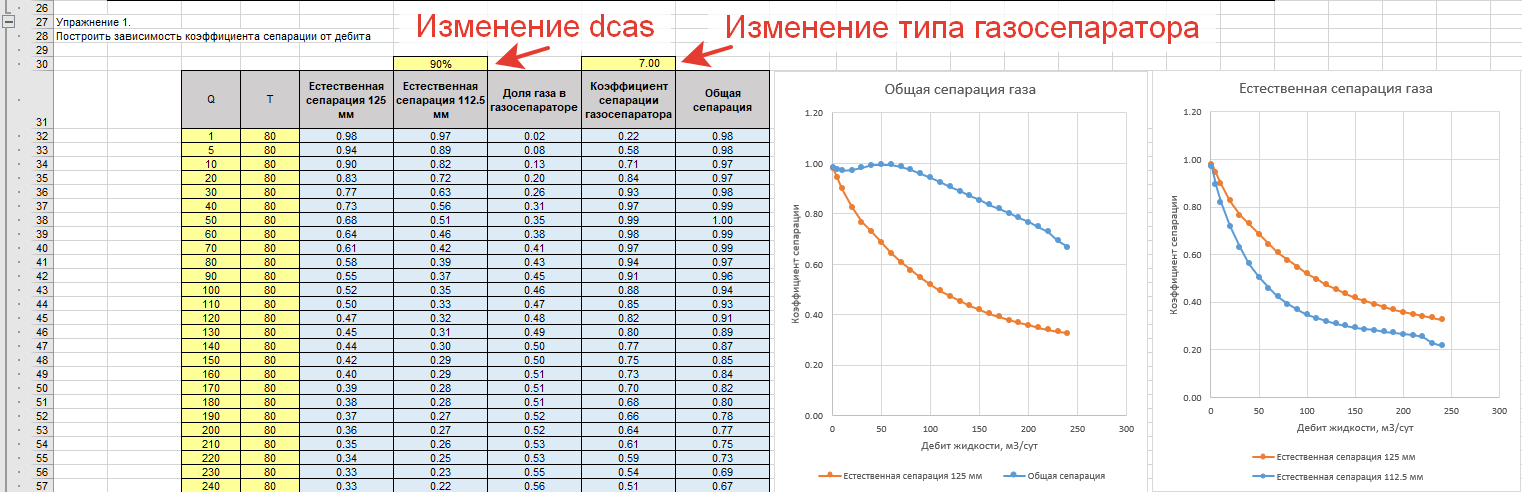
\includegraphics[width=1\linewidth]{Ex60_2}}
	\caption{Результаты расчета естественной и искусственной сепарации}
	\label{ris:Ex60_2}
\end{figure}

Вопросы к упражнению

\begin{enumerate}
	\item От каких параметров будет зависеть коэффициент сепарации?
	\item Как взаимосвязана естественная и искусственная сепарация? 
\end{enumerate}


\section{Анализ работы ЭЦН}

Сегодня доминирующая доля нефти в РФ добывается при помощи ЭЦН. Требуется детальное понимание основных особенностях эксплуатации данного оборудования, режимах работы, возможных осложнениях по причине высокой вязкости продукции, газосодержания, механических примесей и т.д.

Наиболее ценную информацию о работе насоса может дать его характеристика: зависимость параметров работы ЭЦН - напора, потребляемой мощности, перепада давления, КПД, от подачи (дебита скважины)

Для анализа работы скважины, оснащенной УЭЦН, требуются следующие исходные данные

\begin{enumerate}
	\item Физико - химические свойства флюида
	\item Данные по скважине
	\item Данные по ЭЦН
	\item Параметры пласта
\end{enumerate}

PVT свойства задаются аналогично предыдущим упражнениям, а для параметров, характеризующих скважину, приняты следующие обозначения

$H_{mes}$ - глубина скважины измеренная (вдоль ствола скважины), м

$H_{mes}- H_{vert}$ - удлинение ствола скважины, м

$H_{pump}$ - глубина спуска насоса, м

$ID_{cas}$ - внутренний диаметр обсадной колонны, мм

$OD_{tub}$ - внешний диаметр НКТ, мм

$ID_{tub}$ - внутренний диаметр НКТ, мм

$D_{intake}$ - диаметр приемной сетки ЭЦН, мм

$P_{buf}$ - буферное давление, атм

$P_{intake}$ - давление на приеме ЭЦН, атм

$T_{intake}$ - температура на приеме ЭЦН, С

$P_{dis}$ - давление на выкиде ЭЦН, атм

$P_{wf}$ - давление на забое, атм

$Q_{liq}$ - дебит жидкости в поверхностных условиях, м3/сут

$f_w$ - обводненность в поверхностных условиях, \%

\begin{figure}[h!]
	\center{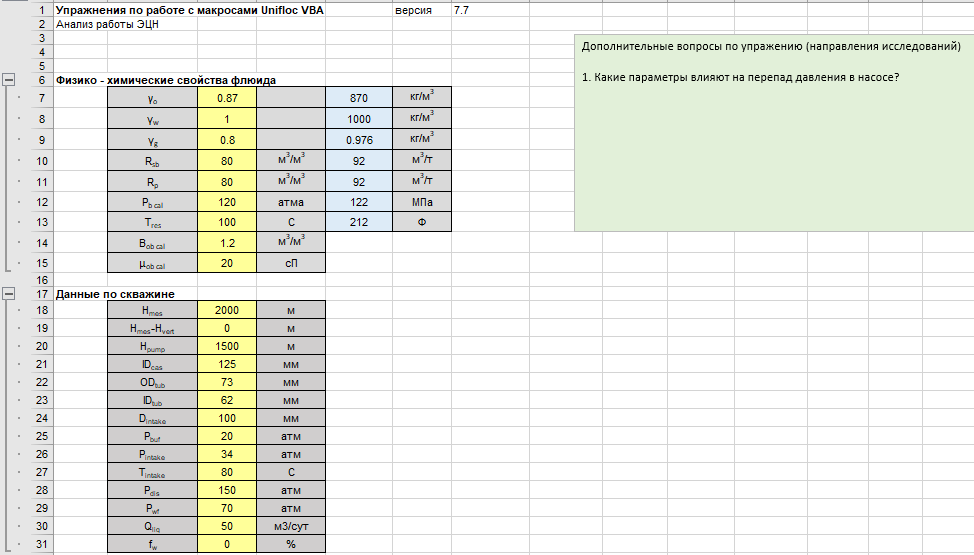
\includegraphics[width=1\linewidth]{Ex70_1}}
	\caption{Исходные данные для свойств флюида и параметров скважины}
	\label{ris:Ex70_1}
\end{figure}

Параметры, описывающие ЭЦН: 

ЭЦН $Q_{nom}$ - номинальная подача ЭЦН, м3/сут

ЭЦН $H_{nom}$ - номинальная напом ЭЦН, м

$F$ - частота питающего тока двигателя, Гц

ЭЦН $ID$ - идентификационный номер насоса (по формуле, см. ниже), находящийся в базе \unf

ЭЦН имя - обозначение насоса: название, габарит и номинальная подача (по формуле, см. ниже)

ЭЦН $Q_{max}$ - максимальная производительность насоса (по формуле, см. ниже), м3/сут

Ступени - количество ступеней, исходя из общего напора ЭЦН и напора одной ступени (по формуле, см. ниже), шт

$K_{sep_ГС}$ - коэффициент сепарации газосепаратора, \%

$P_{sep}$ - давление сепарации, атм

$T_{sep}$ - температура сепарации, С

Данные о пласте:

$P_{res}$ - пластовое давление, атм

$PI$ - коэффициент продуктивности скважины (по формуле, см. выше в упражнении IPR), м3/сут/атм

$\frac{dT}{dL}$ - геотермический градиент, град / 100 м

\begin{figure}[h!]
	\center{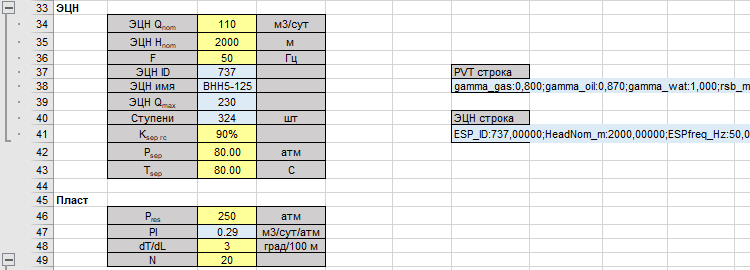
\includegraphics[width=1\linewidth]{Ex70_2}}
	\caption{Исходные данные для ЭЦН и пласта}
	\label{ris:Ex70_2}
\end{figure}

Для получения идентификационного номера насоса в базе \unf \ была использована формула

{ \small  \texttt{=ESP\_id\_by\_rate(Q\_ESP\_)}}

Для определения обозначения ЭЦН

{ \small  \texttt{=ESP\_name(C37)}}

Расчет максимально возможного дебита

{ \small  \texttt{=esp\_max\_rate\_m3day(Freq\_;PumpID\_)*1}}

Количество ступеней

{ \small  \texttt{=ЦЕЛОЕ(Head\_ESP\_/ESP\_head\_m(Q\_ESP\_;1;;PumpID\_))
}}

Также для удобства использования параметры насоса: ID, напор и рабочая частота, зашифровываются в строку с помощью функции

{ \small  \texttt{=ESP\_Encode\_string(PumpID\_;Head\_ESP\_;Freq\_)}}

Свободный газ негативно влияет на работу ЭЦН. В ячейке D51 вычисляется объемная доля газа на приеме газосепаратора с помощью формулы

{ \small  \texttt{=MF\_gas\_fraction\_d(Pintake\_;Tintake\_;fw\_;PVTstr)}}
 
В соседней ячейке D50 для удобного расположения задается вязкость в сПуаз

Построение напорной характеристики данного насоса выполняется с учетом вязкости перекачиваемой продукции. Реализованный метод пересчета характеристики с воды на вязкую жидкость Института Гидравлики позволяет учитывать изменение рабочих параметров из-за данного негативного влияния.

Для вычисления напора в метрах водного столба в ячейке D54 воспользуйтесь формулой

{ \small  \texttt{=ESP\_head\_m(C54;NumStage\_;Freq\_;PumpID\_;mu)}}

КПД ЭЦН в долях единиц 

{ \small  \texttt{=ESP\_eff\_fr(C54;NumStage\_;Freq\_;PumpID\_;mu)}}

Потребляемую ЭЦН мощность в Вт

{ \small  \texttt{=ESP\_Power\_W(C54;NumStage\_;Freq\_;PumpID\_;mu)}}

\begin{figure}[h!]
	\center{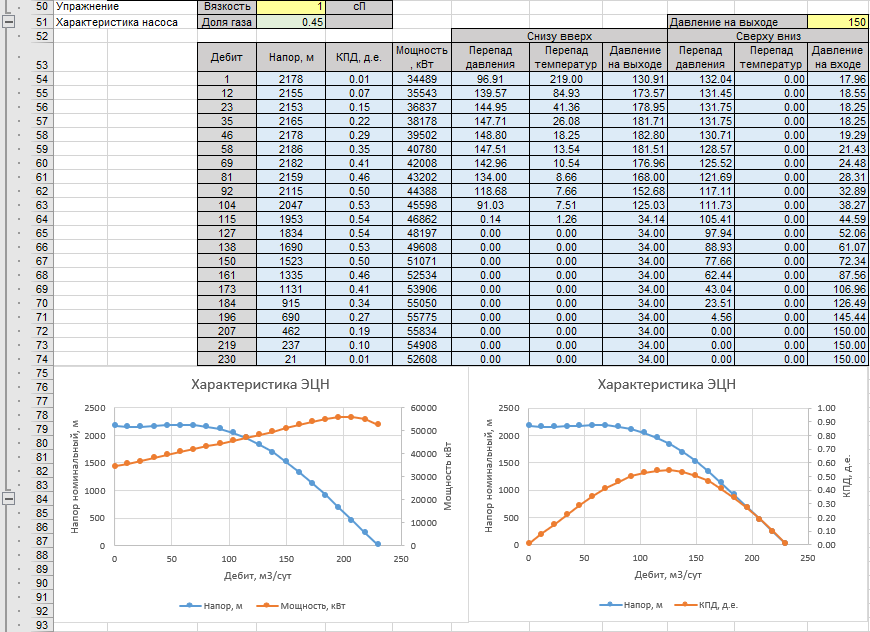
\includegraphics[width=1\linewidth]{Ex70_3}}
	\caption{Напорные характеристики ЭЦН с поправкой на вязкость}
	\label{ris:Ex70_3}
\end{figure}

Расчет перепада давления, развиваемого насосом, может происходить методом "сверху-вниз" \  и "снизу-вверх" \ , при этом расчет перепада температур только методом "снизу-вверх". Функция расчета перепада давления и температуры возвращает массив значений, т.е. одновременно перепад давления и температуры. Кроме того, входным параметром для данной функции является направление расчета. Для вычисления выделите диапазон G54:H54, наберите формулу

{ \small  \texttt{=ESP\_dP\_atm(C54; fw\_; Pintake\_; NumStage\_; Freq\_; PumpID\_; PVTstr; Tintake\_; 0)}}

и после нажмите сочетание клавиш  Ctrl+Shift+Enter. Далее протяните результат до полного заполнения двух столбцов.

Зная давление на приеме и перепад давления в ЭЦН, давление на выходе ЭЦН можно легко посчитать по формуле

{ \small  \texttt{=G54+Pintake\_}}

Предварительно задав давление на выходе ЭЦН в ячейке L51 возможно посчитать перепад давления методом "сверху-вниз"\ аналогичным образом по формуле

{ \small  \texttt{=ESP\_dP\_atm(C54; fw\_; Pdis\_; NumStage\_; Freq\_; PumpID\_; PVTstr; Tintake\_; Tintake\_; 0)}}

И давление на входе, зная давление на выходе и перепад давления

{ \small  \texttt{=Pdis-J54}}

\begin{figure}[h!]
	\center{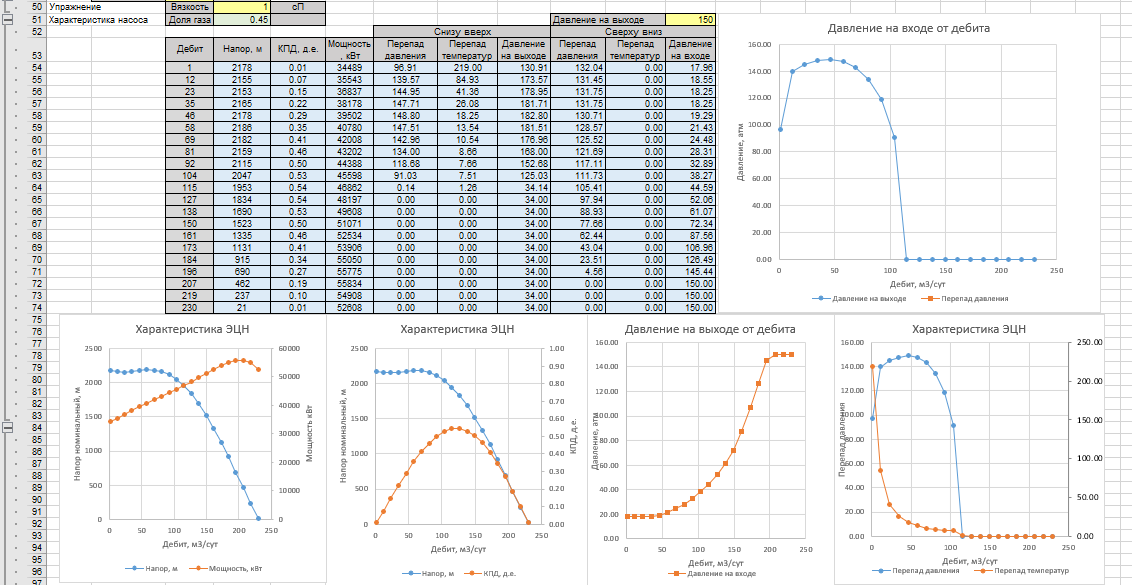
\includegraphics[width=1\linewidth]{Ex70_4}}
	\caption{Расчет перепада давления и температур в ЭЦН в зависимости от дебита}
	\label{ris:Ex70_4}
\end{figure}

Вопросы для упражнения:

\begin{enumerate}
	\item Какие параметры влияют на перепад давления в насосе?
	\item Насколько сильно влияет вязкость на напорные характерситики ЭЦН?
	\item Как влияет на работу ЭЦН изменение частоты?
\end{enumerate}






